\documentclass[12pt,a4paper]{article}
\usepackage[margin=2cm]{geometry}
\usepackage{graphicx} % Required for including pictures
\usepackage{float} % Allows putting an [H] in \begin{figure} to specify the exact location of the figure
\usepackage{wrapfig} % Allows in-line images such as the example fish picture
\usepackage{color}
\usepackage{mathtools}
\usepackage{graphicx}
\usepackage{hyperref}
\usepackage{titling}
\usepackage{braket}
\usepackage{cancel}
\usepackage{acronym}
\usepackage{subcaption}
\usepackage{caption}
\usepackage[space]{grffile} % allows file names with spaces
\usepackage{lipsum}

\hypersetup{
colorlinks=true,
linkcolor=blue,
urlcolor=blue
}

\acrodef{stem}[STEM]{Scanning Transmission Electron Microscopy}
\acrodef{tem}[TEM]{Transmission Electron Microscope}
\acrodef{cemn}[CEMN]{Center for Electron Microscopy and Nanofabrication}
\acrodef{edx}[EDX]{Energy-dispersive X-ray spectroscopy}
\acrodef{sem}[SEM]{Scanning Electron Microscope}
% http://staff.science.uva.nl/~polko/HOWTO/LATEX/acronym.html 

%\setlength\parindent{0pt} % Uncomment to remove all indentation from paragraphs

\graphicspath{{Data/}} % Specifies the directory where pictures are stored

\title{TEM Report 2}
\author{Bret Comnes}
\date{\today}
\posttitle{\par\end{center}}
\setlength{\droptitle}{-10pt}


\begin{document}

\maketitle

\section{Introduction} % Major section

This report will cover some basics concepts relating to \ac{stem} and \ac{edx}, as well as some simple analysis of data taken a student lab session at the \ac{cemn} at Portland State University on May 16, 2014.  Bright field \ac{stem} images, \ac{edx} data and point spectrum of the inspected sample are included.  The data was collected using a FEI Technai \ac{tem} and the accompanying AZtec EDS acquisition and analysis tool.

Spectrum analysis is performed using last available freely distributed version of Fityk\cite{ft}: v.1.2.9.  Additional work was performed to build newer versions of Fityk from source and add it to the Homebrew\cite{home} package manager for future convenience of other students and researches.


\section{\ac{stem} Fundamentals} % (fold)
\label{sec:stem}

\ac{stem} uses the formation of a fine point of electrons rastering across the sample to provide information about specific points of the specimen.  This allows for mapping of \ac{edx} to specific points of the sample as well as limiting radiation exposure to smaller well defined sections of the sample.  Scanning coils are used to horizontally scan the beam across the surface as apposed to pivoting around a point like you would find in an \ac{sem}.

Because \ac{stem} images are formed by a raster scan, instead of using lenses to form an image, we no longer have to worry about defects in our lenses which can cause issues like chromatic aberration in thick samples.  Magnification of \ac{stem} images are determined by scan geometry.  While \ac{stem} can provide better contrast, images tend to be noisier than \ac{tem} mode images.  \cite{tem}  

\ac{stem} can generate both bright field and dark field images.  \ac{stem} actually provides images with less noise and better contrast than \ac{tem} but at the cost of lower resolution.  This can be useful for thick or unstained samples which provide very little image details and require the higher contrast \ac{stem} provides.  \ac{stem} gives more flexibility over the contrast of images because it allows control over things like detector gain and contrast/brightness settings that are not available on the analog \ac{tem} screen  (however you can always digitalis images from the normal \ac{tem} mode and apply post processing to your images to enhance contrast).  

\section{\ac{edx} fundamentals} % (fold)
\label{sec:edx}

\ac{edx} allows for detection of the chemical composition of samples.  It can be used with \ac{stem} to map chemical composition to specific locations on the sample.  Electrons are a type of ionizing radiation, meaning, that it can cause inner shell electrons in the sample to be ejected, resulting in secondary signals that contain useful information.  \ac{edx} uses the secondary X-rays ejected due to \ac{tem} radiation to plot the characteristic peaks of the elements contained within a sample.   

\ac{edx} is a form of spectroscopy, so detects and distinguishes x-rays by their energy level.  This is critical for the function of \ac{edx} as the whole point is to determine chemical composition.  Typical detectors are made out of $Si(Li)$.

The probability of an electron in the \ac{tem} beam ionizing an atom if your sample is dependent upon the ionization cross section.
% section acedx_fundamentals (end)

\section{Data Analysis} % (fold)
\label{sec:data_analysis}

We collected bright field TEM images of a Iron Oxide ($Fe_3O_4$) particles coated with Silicon dioxide ($SiO_2$).  Additionally, we collected \ac{edx} spectrum information and mapped the location of these different elements using the AZtec software.  The data was explored in a limited manner use the Fityk software.  Unfortunately the \ac{stem} images were lost in the process of exporting data and cannot be included.

\subsection{TEM imaging} % (fold)
\label{sub:tem_imaging}

Bright field images of Iron Oxide particles coated with Silicon dioxide were taken.  \ac{tem} imaging consists of illuminating thin samples that are semi electron transparent with a focused electron beam to project an image of the sample onto a viewing screen or camera.

\lipsum[6] % Dummy text

\begin{figure}[htbp]
  \centering
  
  \begin{subfigure}[b]{0.45\textwidth}
    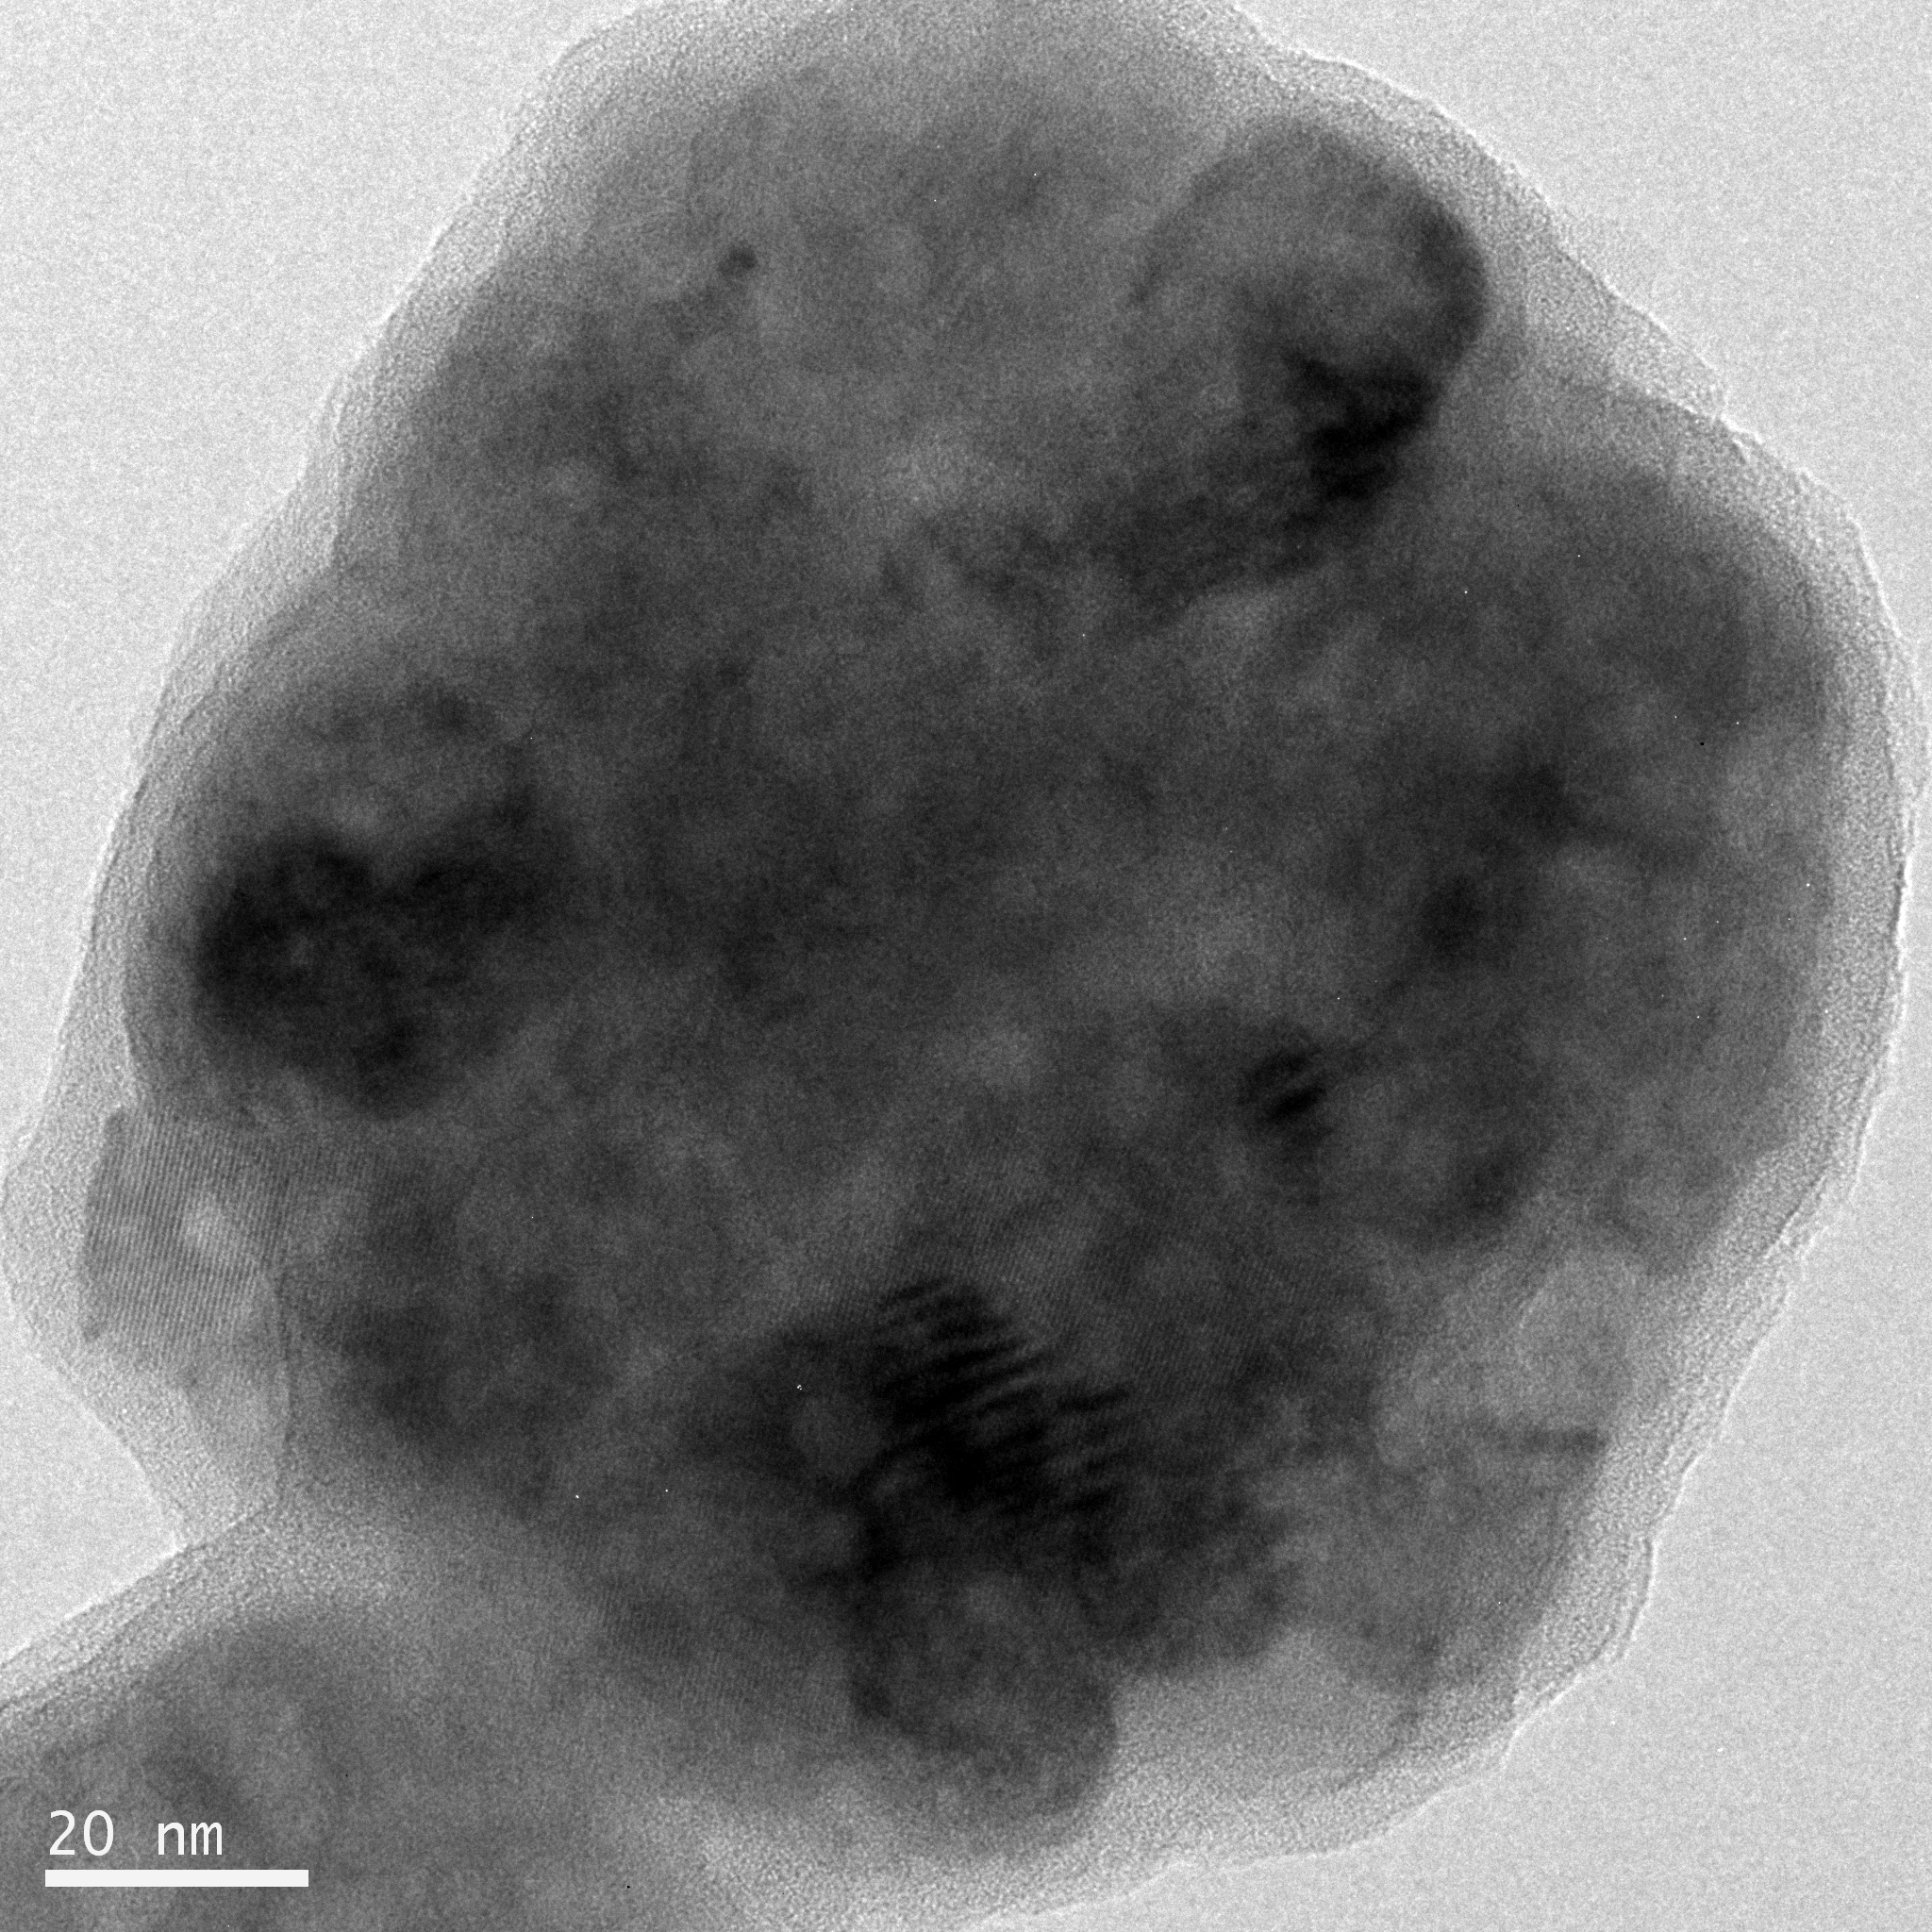
\includegraphics[width=\textwidth]{Data/Fe3O4-SiO2-0001.png}
  \end{subfigure}%
  \begin{subfigure}[b]{0.45\textwidth}
    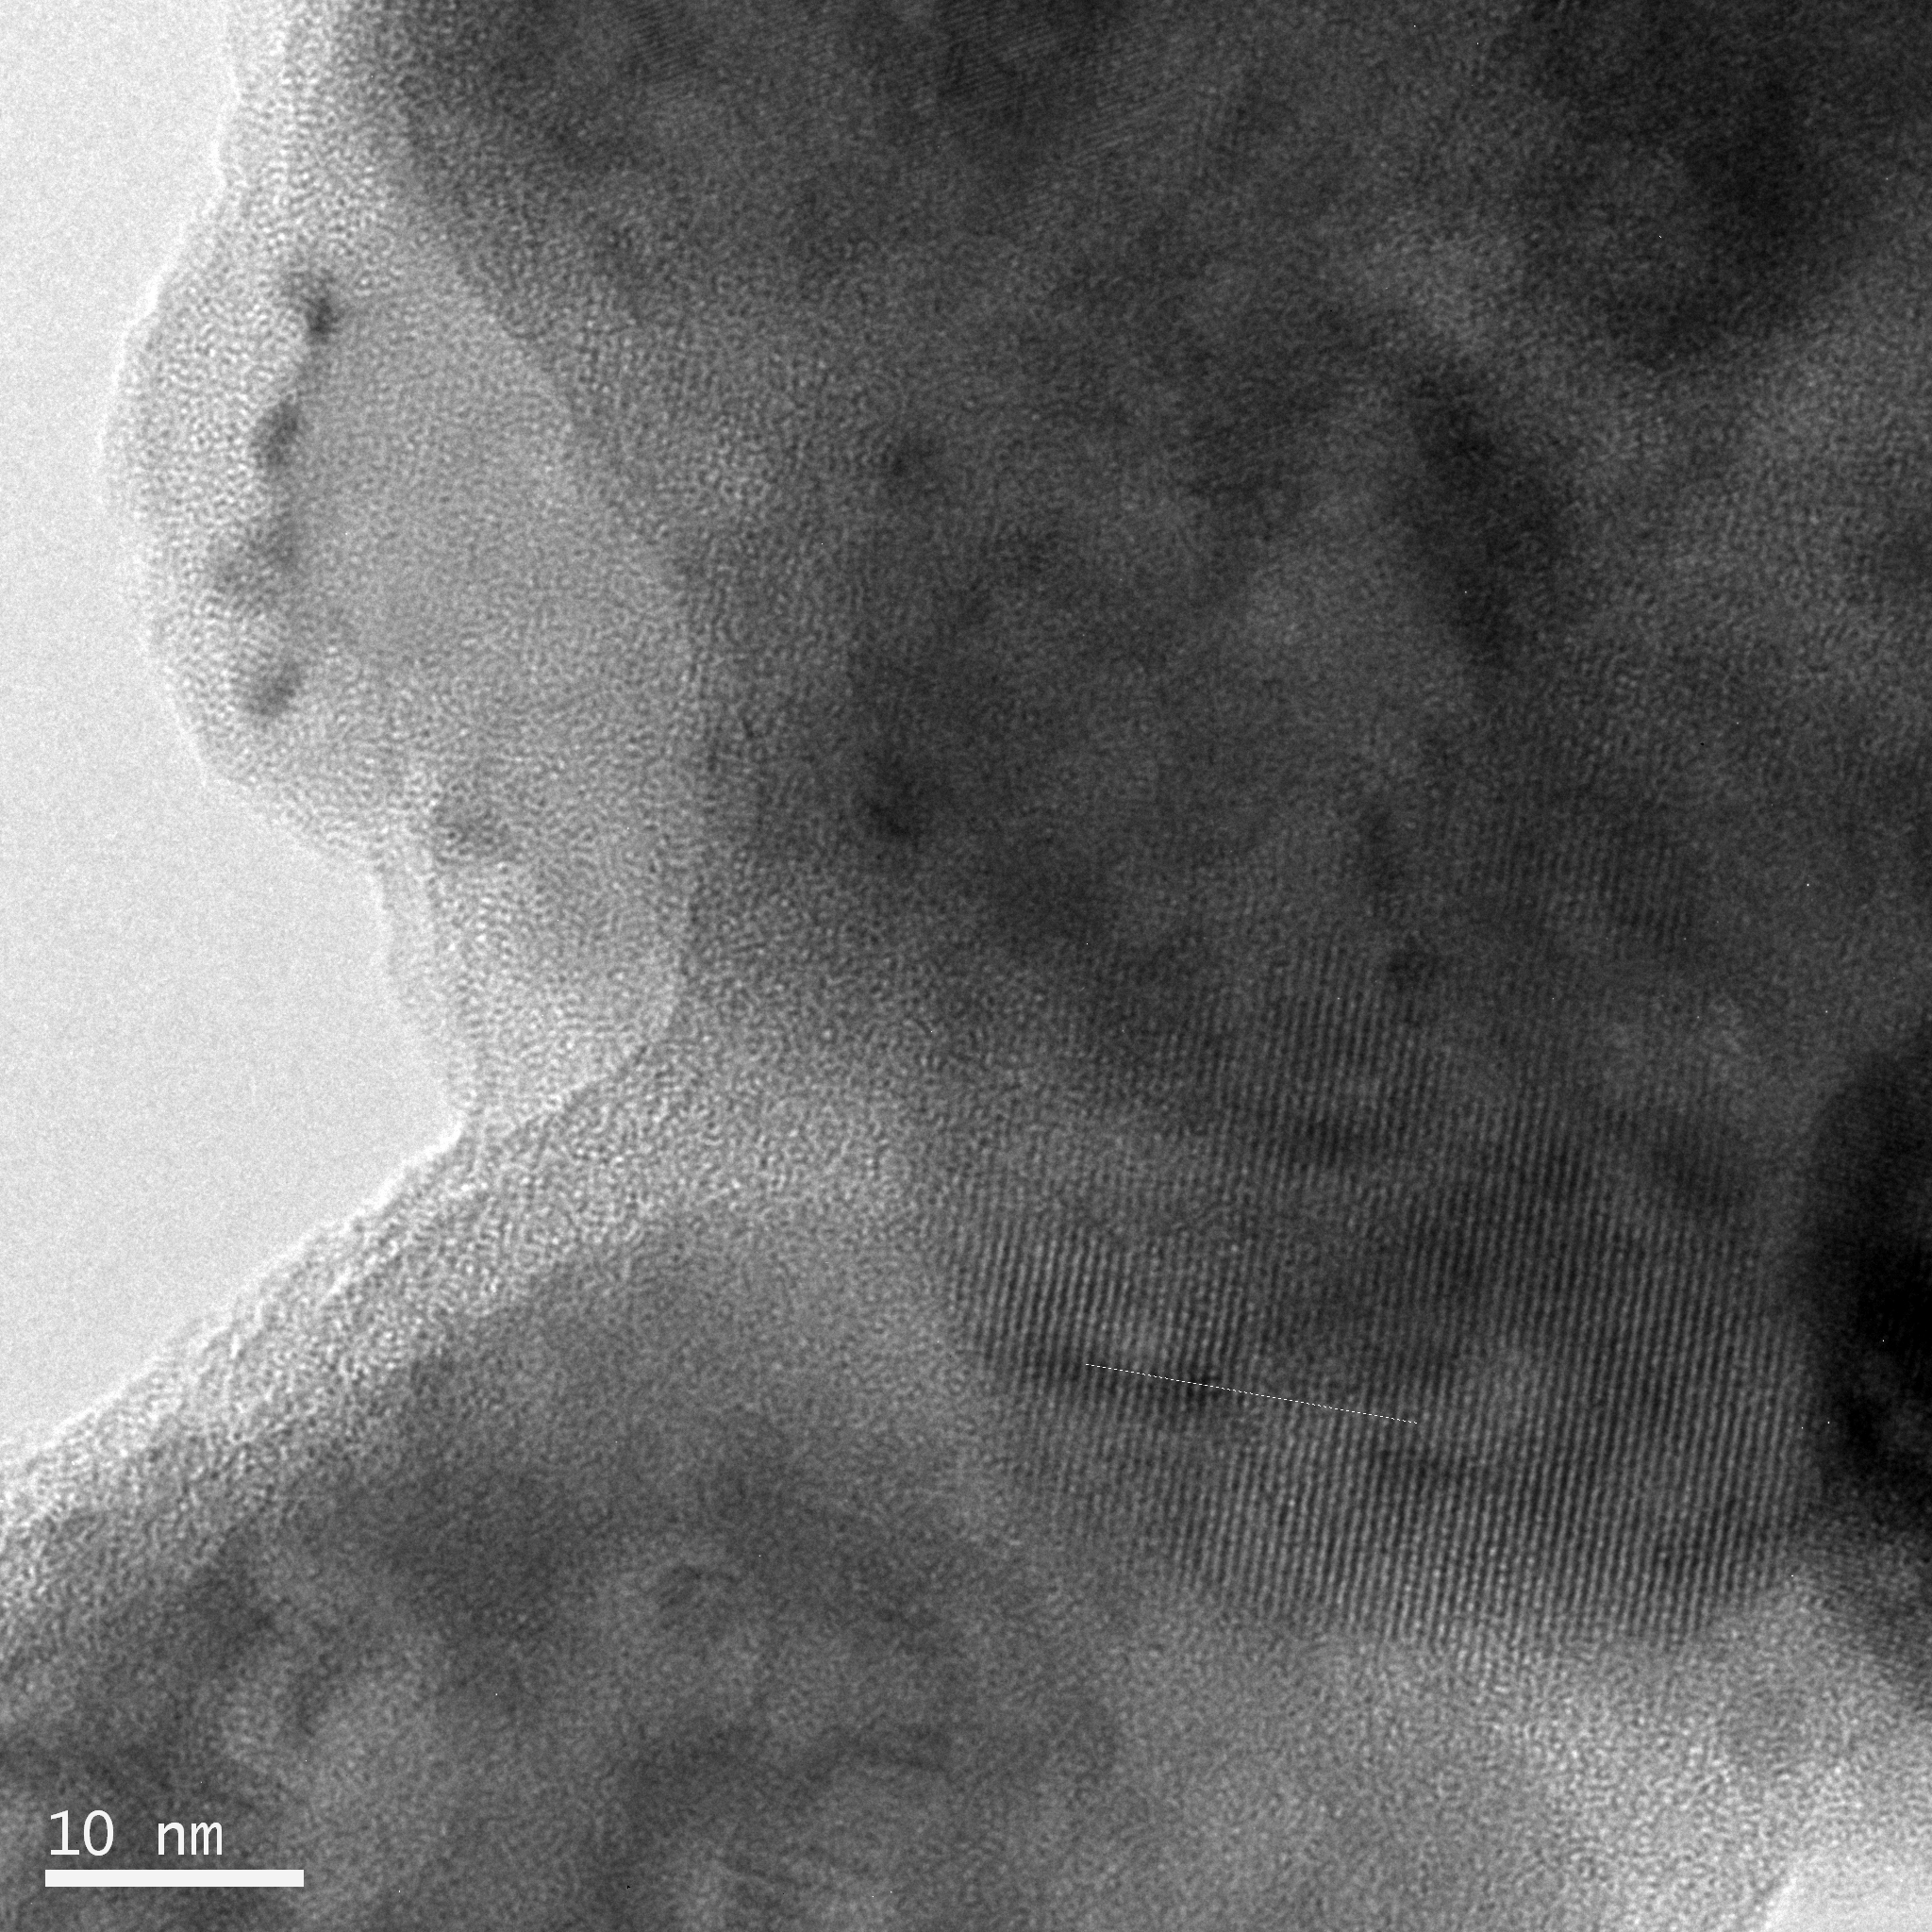
\includegraphics[width=\textwidth]{Data/Fe3O4-SiO2-0002.png}
  \end{subfigure}
  
  \begin{subfigure}[b]{0.45\textwidth}
    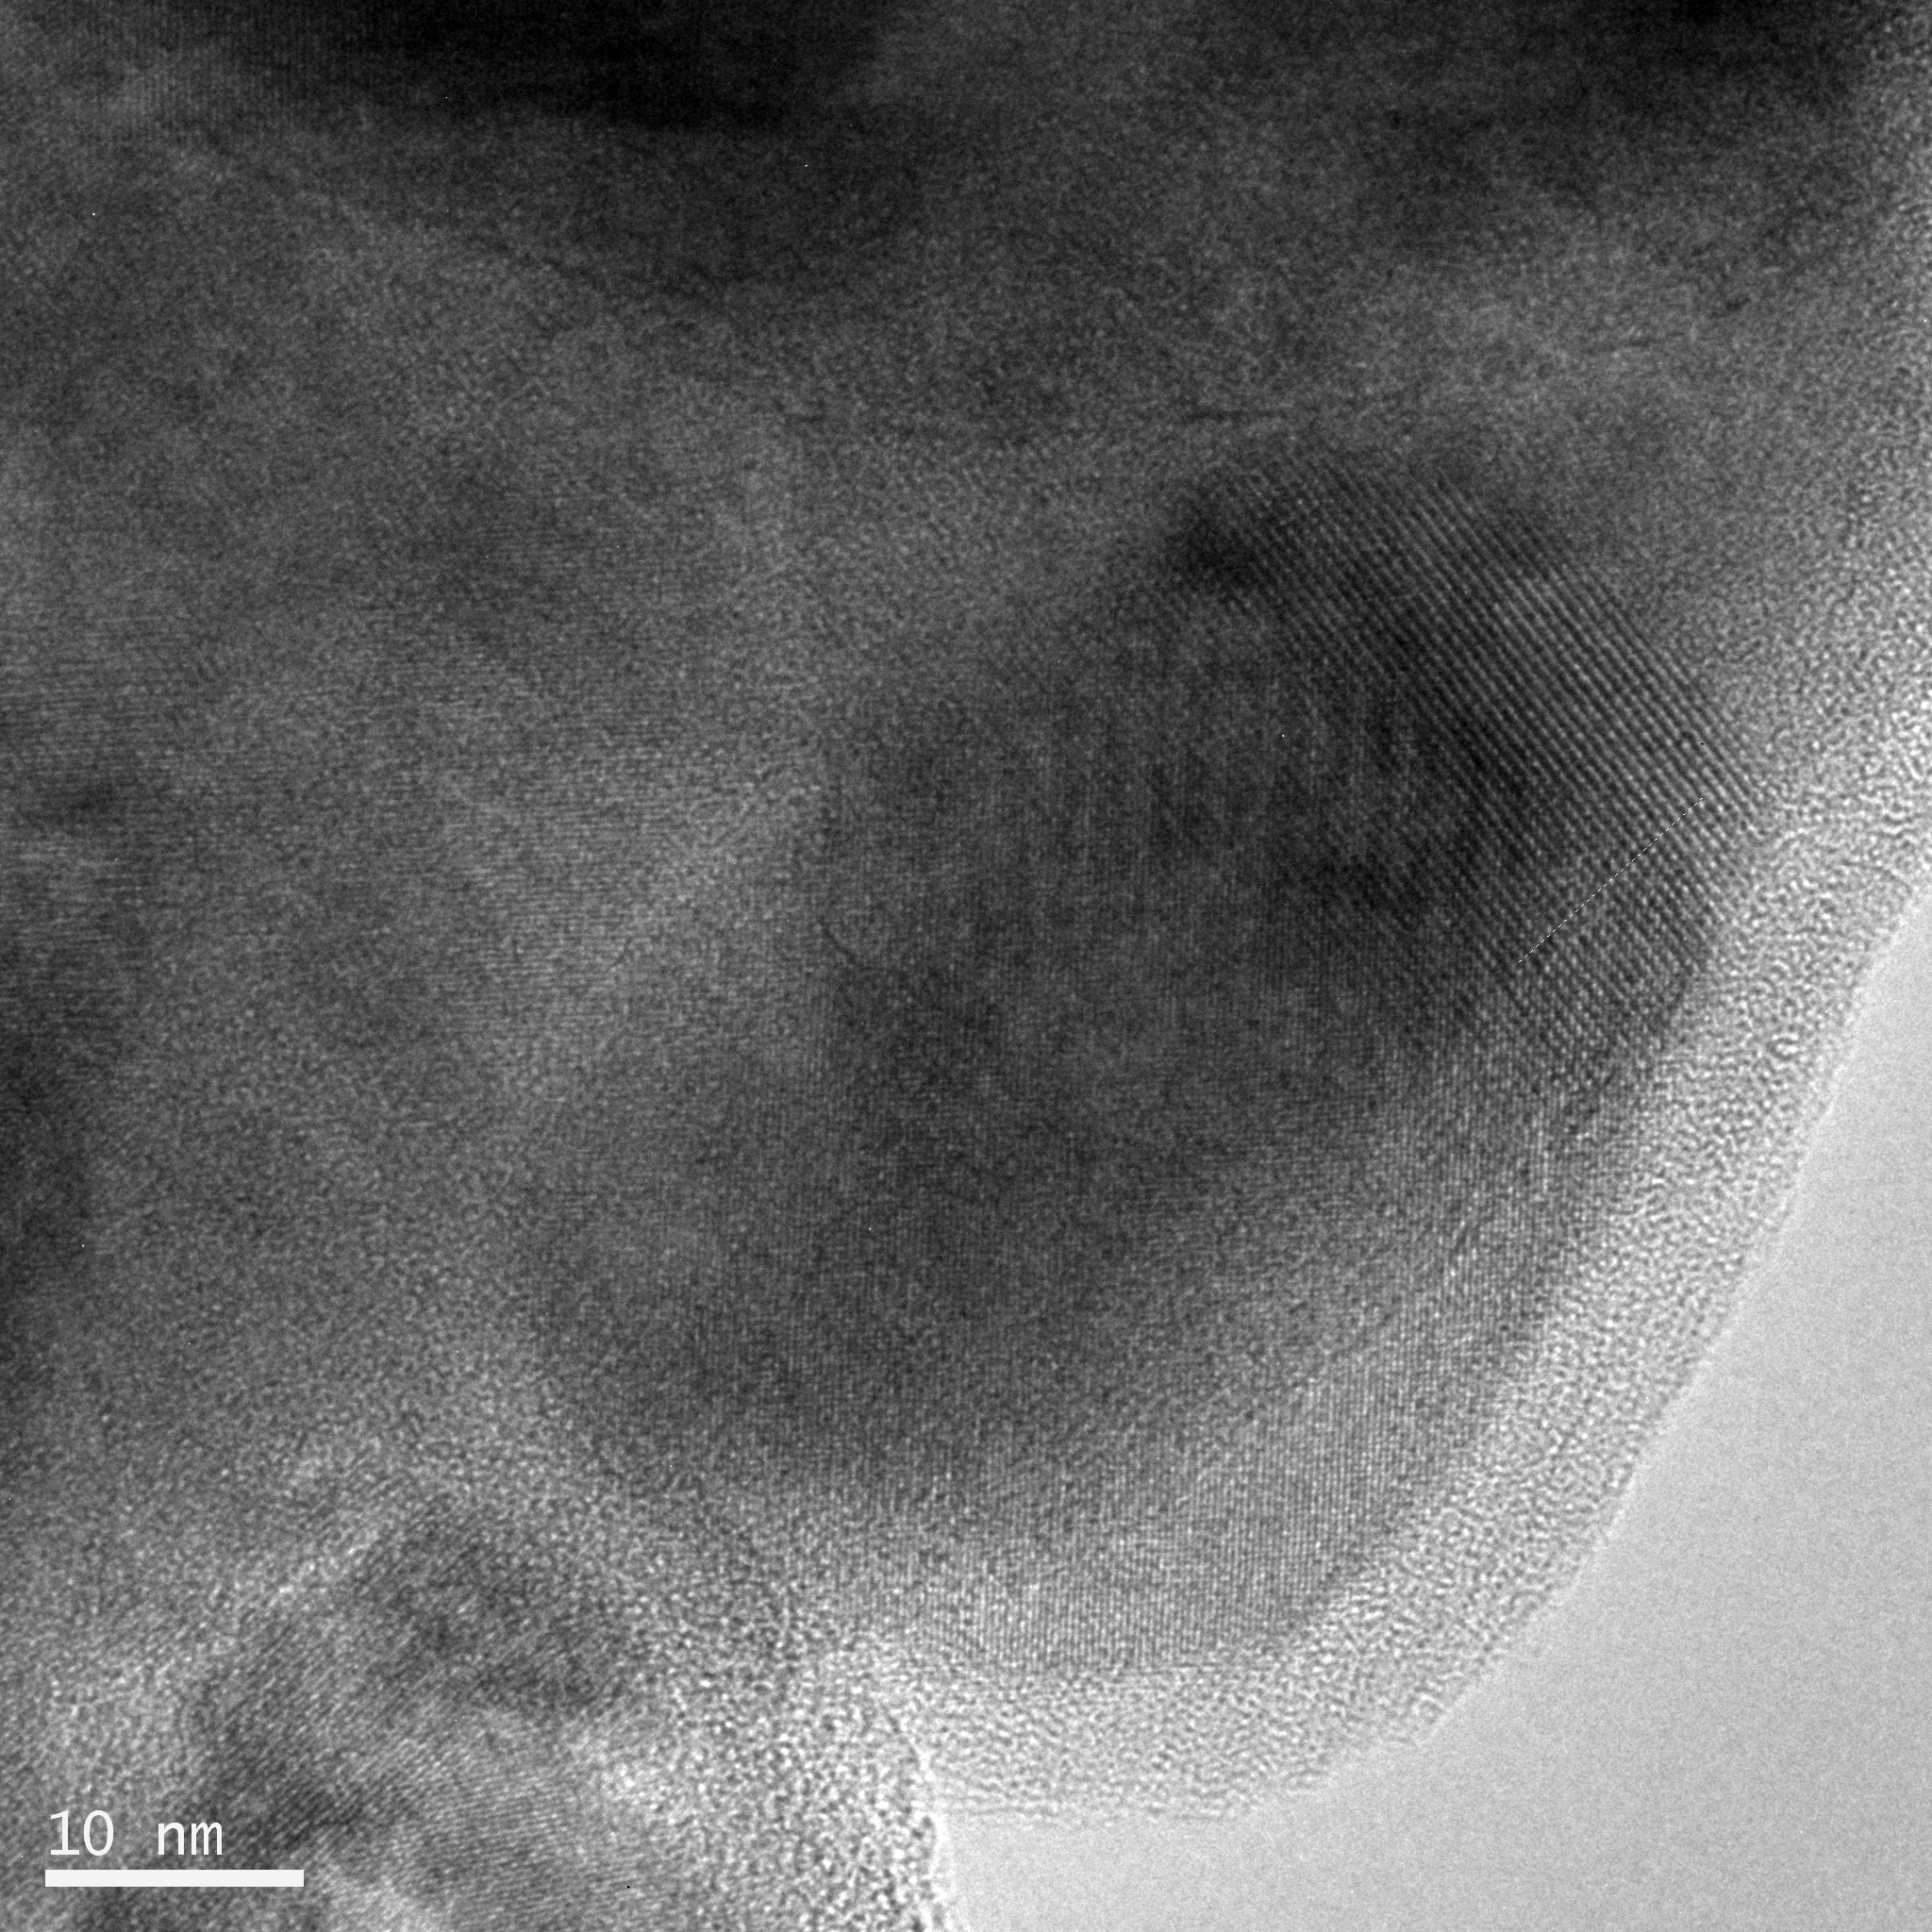
\includegraphics[width=\textwidth]{Data/Fe3O4-SiO2-0003.png}
    \caption{Visible lattice pattern}
    \label{fig:viewc}
  \end{subfigure}
  \begin{subfigure}[b]{0.45\textwidth}
    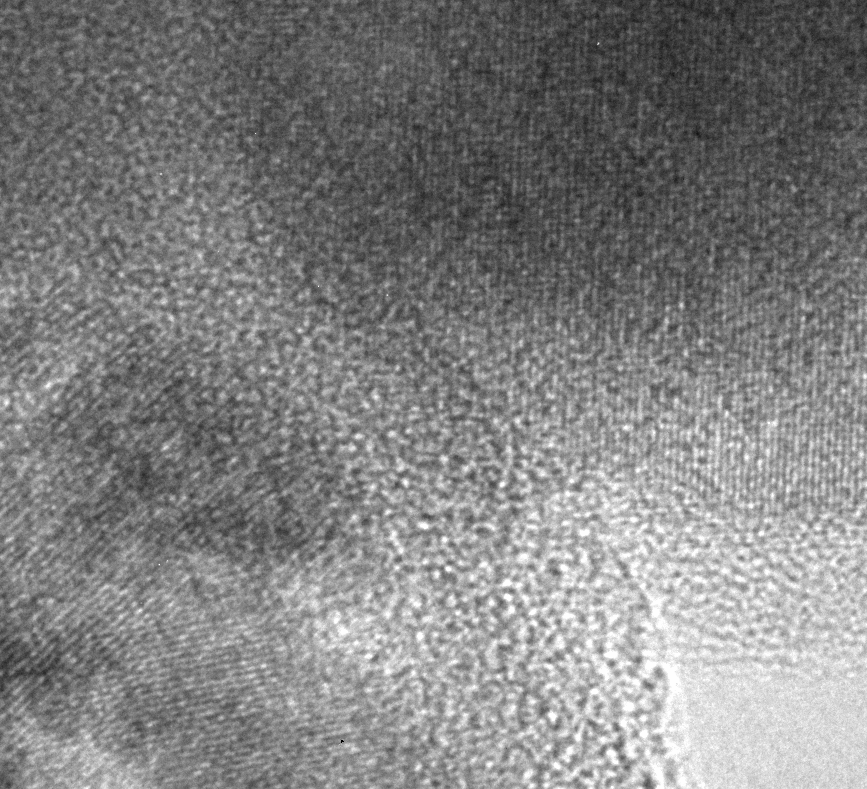
\includegraphics[width=\textwidth]{Data/Fe3O4-SiO2-0003-zoom.png}
    \caption{Magnified view of \ref{fig:viewc}.  }
    \label{fig:zoom}
  \end{subfigure}
  
  \caption{Various views of Bright field Images of $SiO_2$ coated $Fe_3O_4$ particles}\label{fig:brightfield}
\end{figure}

% subsection tem_imaging (end)

\subsection{EDX Spectroscopy} % (fold)
\label{sub:edx_spectroscopy}

\lipsum[6] % Dummy text

\lipsum[6] % Dummy text

\lipsum[6] % Dummy text

\begin{wrapfigure}{r}{0.5\textwidth}
  \begin{subfigure}[b]{0.5\textwidth}
    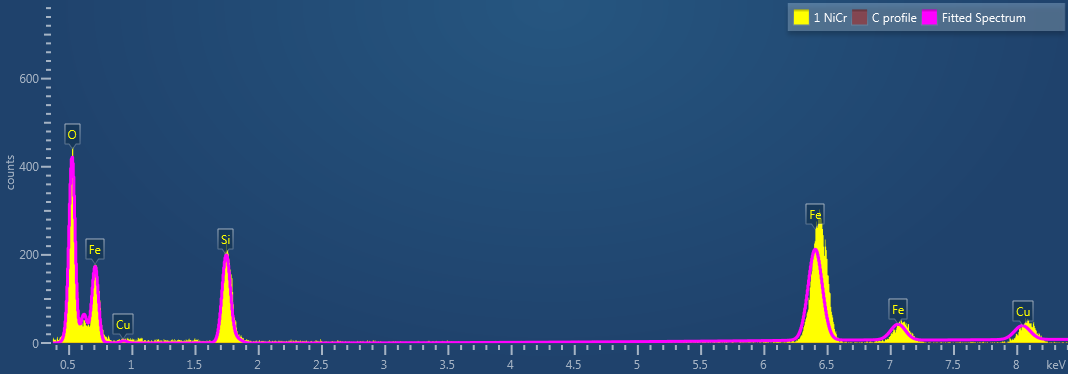
\includegraphics[width=\textwidth]{Data/EDS Spectrum.png}
    \caption{EDX Spectrum from AZtec}
    \label{fig:aztec}
  \end{subfigure}%

  \begin{subfigure}[b]{0.5\textwidth}
    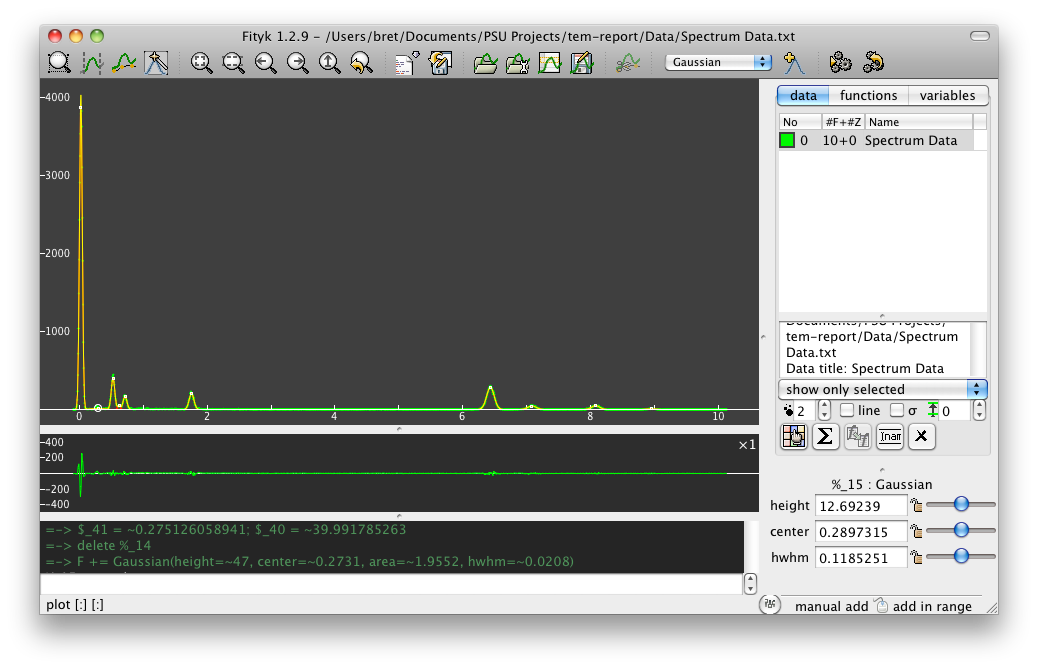
\includegraphics[width=\textwidth]{Data/full.png}
    \caption{Fitted EDX Spectrum from Fityk}
    \label{fig:fitk}
  \end{subfigure}%

  \caption{EDX Spectroscopy Data}
  \label{fig:edx}
\end{wrapfigure}

\begin{figure}[htbp]
  \centering
    \begin{subfigure}[b]{0.45\textwidth}
    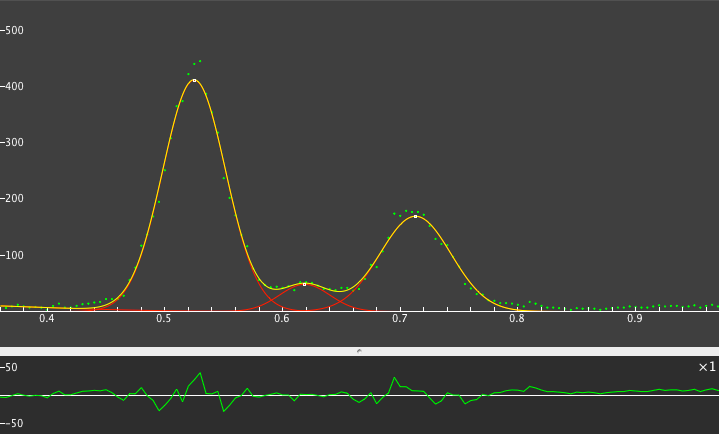
\includegraphics[width=\textwidth]{Data/crossover.png}
    \caption{False peak between $Fe$ and $Cu$ peaks.}
    \label{fig:cross}
  \end{subfigure}
  ~
  \begin{subfigure}[b]{0.45\textwidth}
    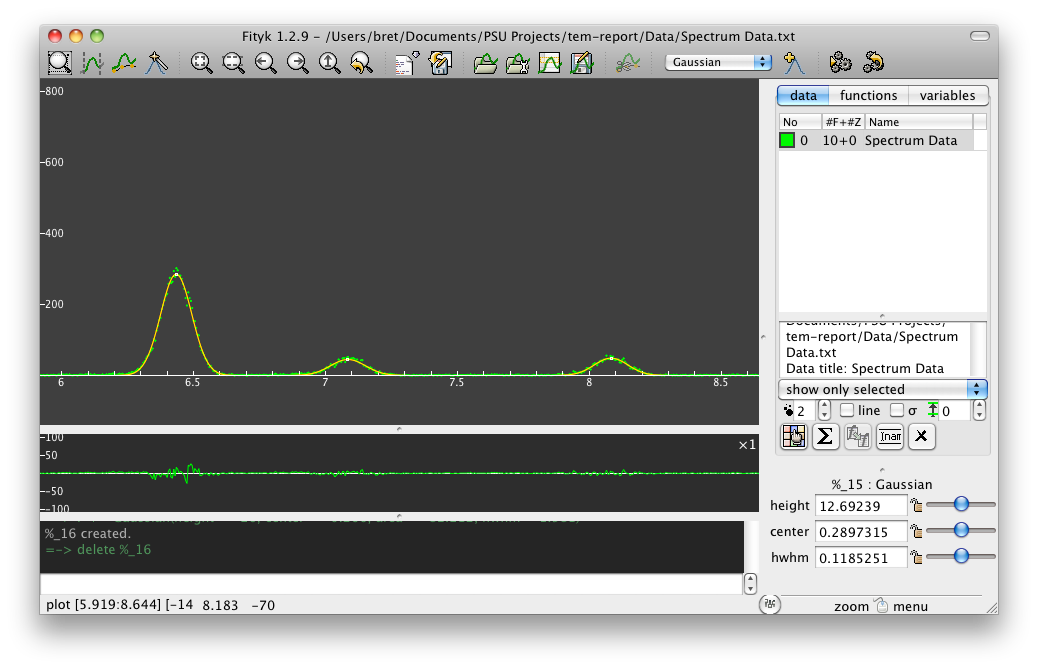
\includegraphics[width=\textwidth]{Data/outer_peak.png}
    \caption{Close up of outer $Fe$ and $Cu$ peaks.}
    \label{fig:outer}
  \end{subfigure}%
  \caption{Close up of fitted data in Fityk}
  \label{fig:fit}
\end{figure}

% subsection edx_spectroscopy (end)

\subsection{EDS Maps} % (fold)
\label{sub:eds_maps}

\lipsum[6] % Dummy text

\lipsum[6] % Dummy text

\lipsum[6] % Dummy text

\begin{figure}[htbp]
  \centering
  \begin{subfigure}[b]{0.35\textwidth}
    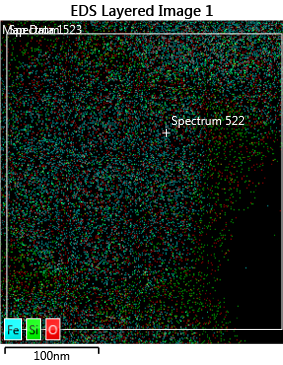
\includegraphics[width=\textwidth]{Data/Map.png}
    \caption{Composite Element Map}
    \label{fig:map}
  \end{subfigure}
  \begin{subfigure}[b]{0.35\textwidth}
    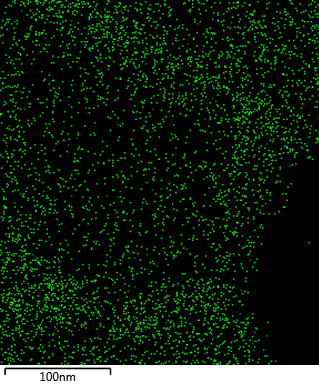
\includegraphics[width=\textwidth]{Data/Si Map.png}
    \caption{Map of $Si$}
    \label{fig:si_map}
  \end{subfigure}

  \begin{subfigure}[b]{0.35\textwidth}
    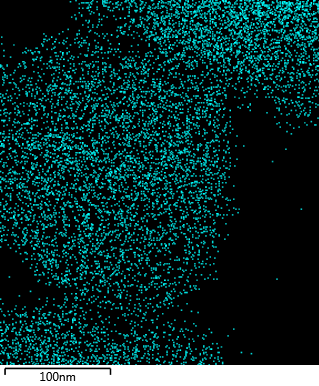
\includegraphics[width=\textwidth]{Data/Fe Map.png}
    \caption{Map of $Fe$}
    \label{fig:fe_map}
  \end{subfigure}
  \begin{subfigure}[b]{0.35\textwidth}
    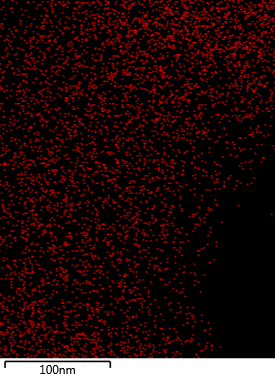
\includegraphics[width=\textwidth]{Data/O Map.png}
    \caption{Map of $O$}
    \label{fig:o_map}
  \end{subfigure}
  \caption{EDX Maps of Particle Sample}\label{fig:map_grid}
\end{figure}

% subsection eds_maps (end)

% section data_analysis (end)

\section{Fityk Added to Homebrew} % (fold)
\label{sec:fityk_homebrew}

Upon discovering that newer Fityk versions were only offered as runnable binaries for paying subscribers, a simple \texttt{ruby} formula was submitted as a pull request to the Homebrew Science repository\cite{hbs}.  Homebrew\cite{home} is a popular 3rd party package manager for Mac OS X that manages the building and installation of open source software packages.  Upon the writing of this paper, the pull request was waiting for approval discussions with maintainers about acceptance sounded positive\cite{fpr}.  This will allow others to simply install the latest version of Fityk from the command line by running \texttt{\$ brew install fityk}.  A formula for the Fityk dependency, \texttt{xylib}, was also submitted to the \texttt{homebrew-science} repository\cite{xpr}.

% section fityk_homebrew (end)

\section{Conclusion} % Major section

\lipsum[6] % Dummy text

\lipsum[6] % Dummy text

\lipsum[6] % Dummy text

\bibliography{main} 
\bibliographystyle{plain} \nocite{*}

\end{document}